\
\documentclass[reprint,aps,prl,showkeys,amsmath,amssymb,floatfix]{revtex4-2}
\usepackage{graphicx}
\usepackage[colorlinks=true,linkcolor=blue,citecolor=blue,urlcolor=blue]{hyperref}
\begin{document}

\title{A testable brane-world unification with early-time $\rho^2$ and dark radiation}
\author{Ricardo Maldonado}
\email{sales@rank.vegas}
\date{\today}

\begin{abstract}
From a higher-dimensional brane setup we obtain the Shiromizu--Maeda--Sasaki effective equations. In flat FRW, the Friedmann relation becomes
$H^2=\frac{8\pi G}{3}\rho\!\left(1+\frac{\rho}{2\lambda}\right)+\frac{\Lambda_4}{3}+\frac{\mathcal{C}}{a^{4}}$,
featuring a $\rho^2$ correction and a dark-radiation term. A single parameter---the brane tension $\lambda$---predicts a gravitational-wave spectral break $f_{\rm br}\propto \lambda^{1/4}$ and correlates with $\Delta N_{\rm eff}$, yielding a falsifiable joint test using PTA$\to$LISA and CMB/BBN. Using the official NANOGrav 15-yr KDE spectrum with a Planck-2018 $N_{\rm eff}$ prior we present posteriors and a PTA$\to$LISA context figure; the late-time limit reduces to GR.
\end{abstract}

\maketitle

\paragraph{Framework.} In a spatially flat FRW universe the effective equation reads
\begin{equation}
H^2=\frac{8\pi G}{3}\,\rho\!\left(1+\frac{\rho}{2\lambda}\right)+\frac{\Lambda_4}{3}+\frac{\mathcal{C}}{a^{4}}\,,\label{eq:frw}
\end{equation}
with $\lambda$ the brane tension and ${\cal C}/a^4$ the projected Weyl (``dark radiation'') term. The $\rho^2$ piece controls the early-time expansion $a(t)\propto t^{1/4}$. Two test links are
\begin{equation}
f_{\rm br}\propto \lambda^{1/4},\qquad \frac{\mathcal{C}}{\rho_{\gamma,0}}=\frac{7}{8}\left(\frac{4}{11}\right)^{4/3}\Delta N_{\rm eff}\,.
\end{equation}

\paragraph{Data and method.} We convert the official NANOGrav 15-yr KDE free-spectrum to CSV and impose a Planck-2018 prior on $N_{\rm eff}$. Posteriors are obtained on $(\lambda,\Delta N_{\rm eff})$ and compared to LISA sensitivity (instrument vs.\ instrument+confusion variants).

\begin{figure}[t]
  \centering
  \includegraphics[width=0.46\textwidth]{figures/posterior_2D.png}
  \caption{Posterior in $(\lambda,\Delta N_{\rm eff})$.}
\end{figure}

\begin{figure}[t]
  \centering
  \includegraphics[width=0.46\textwidth]{figures/PTA_fit_preview_rebuilt.png}
  \caption{PTA fit preview (MAP vs spectrum points).}
\end{figure}

\begin{figure}[t]
  \centering
  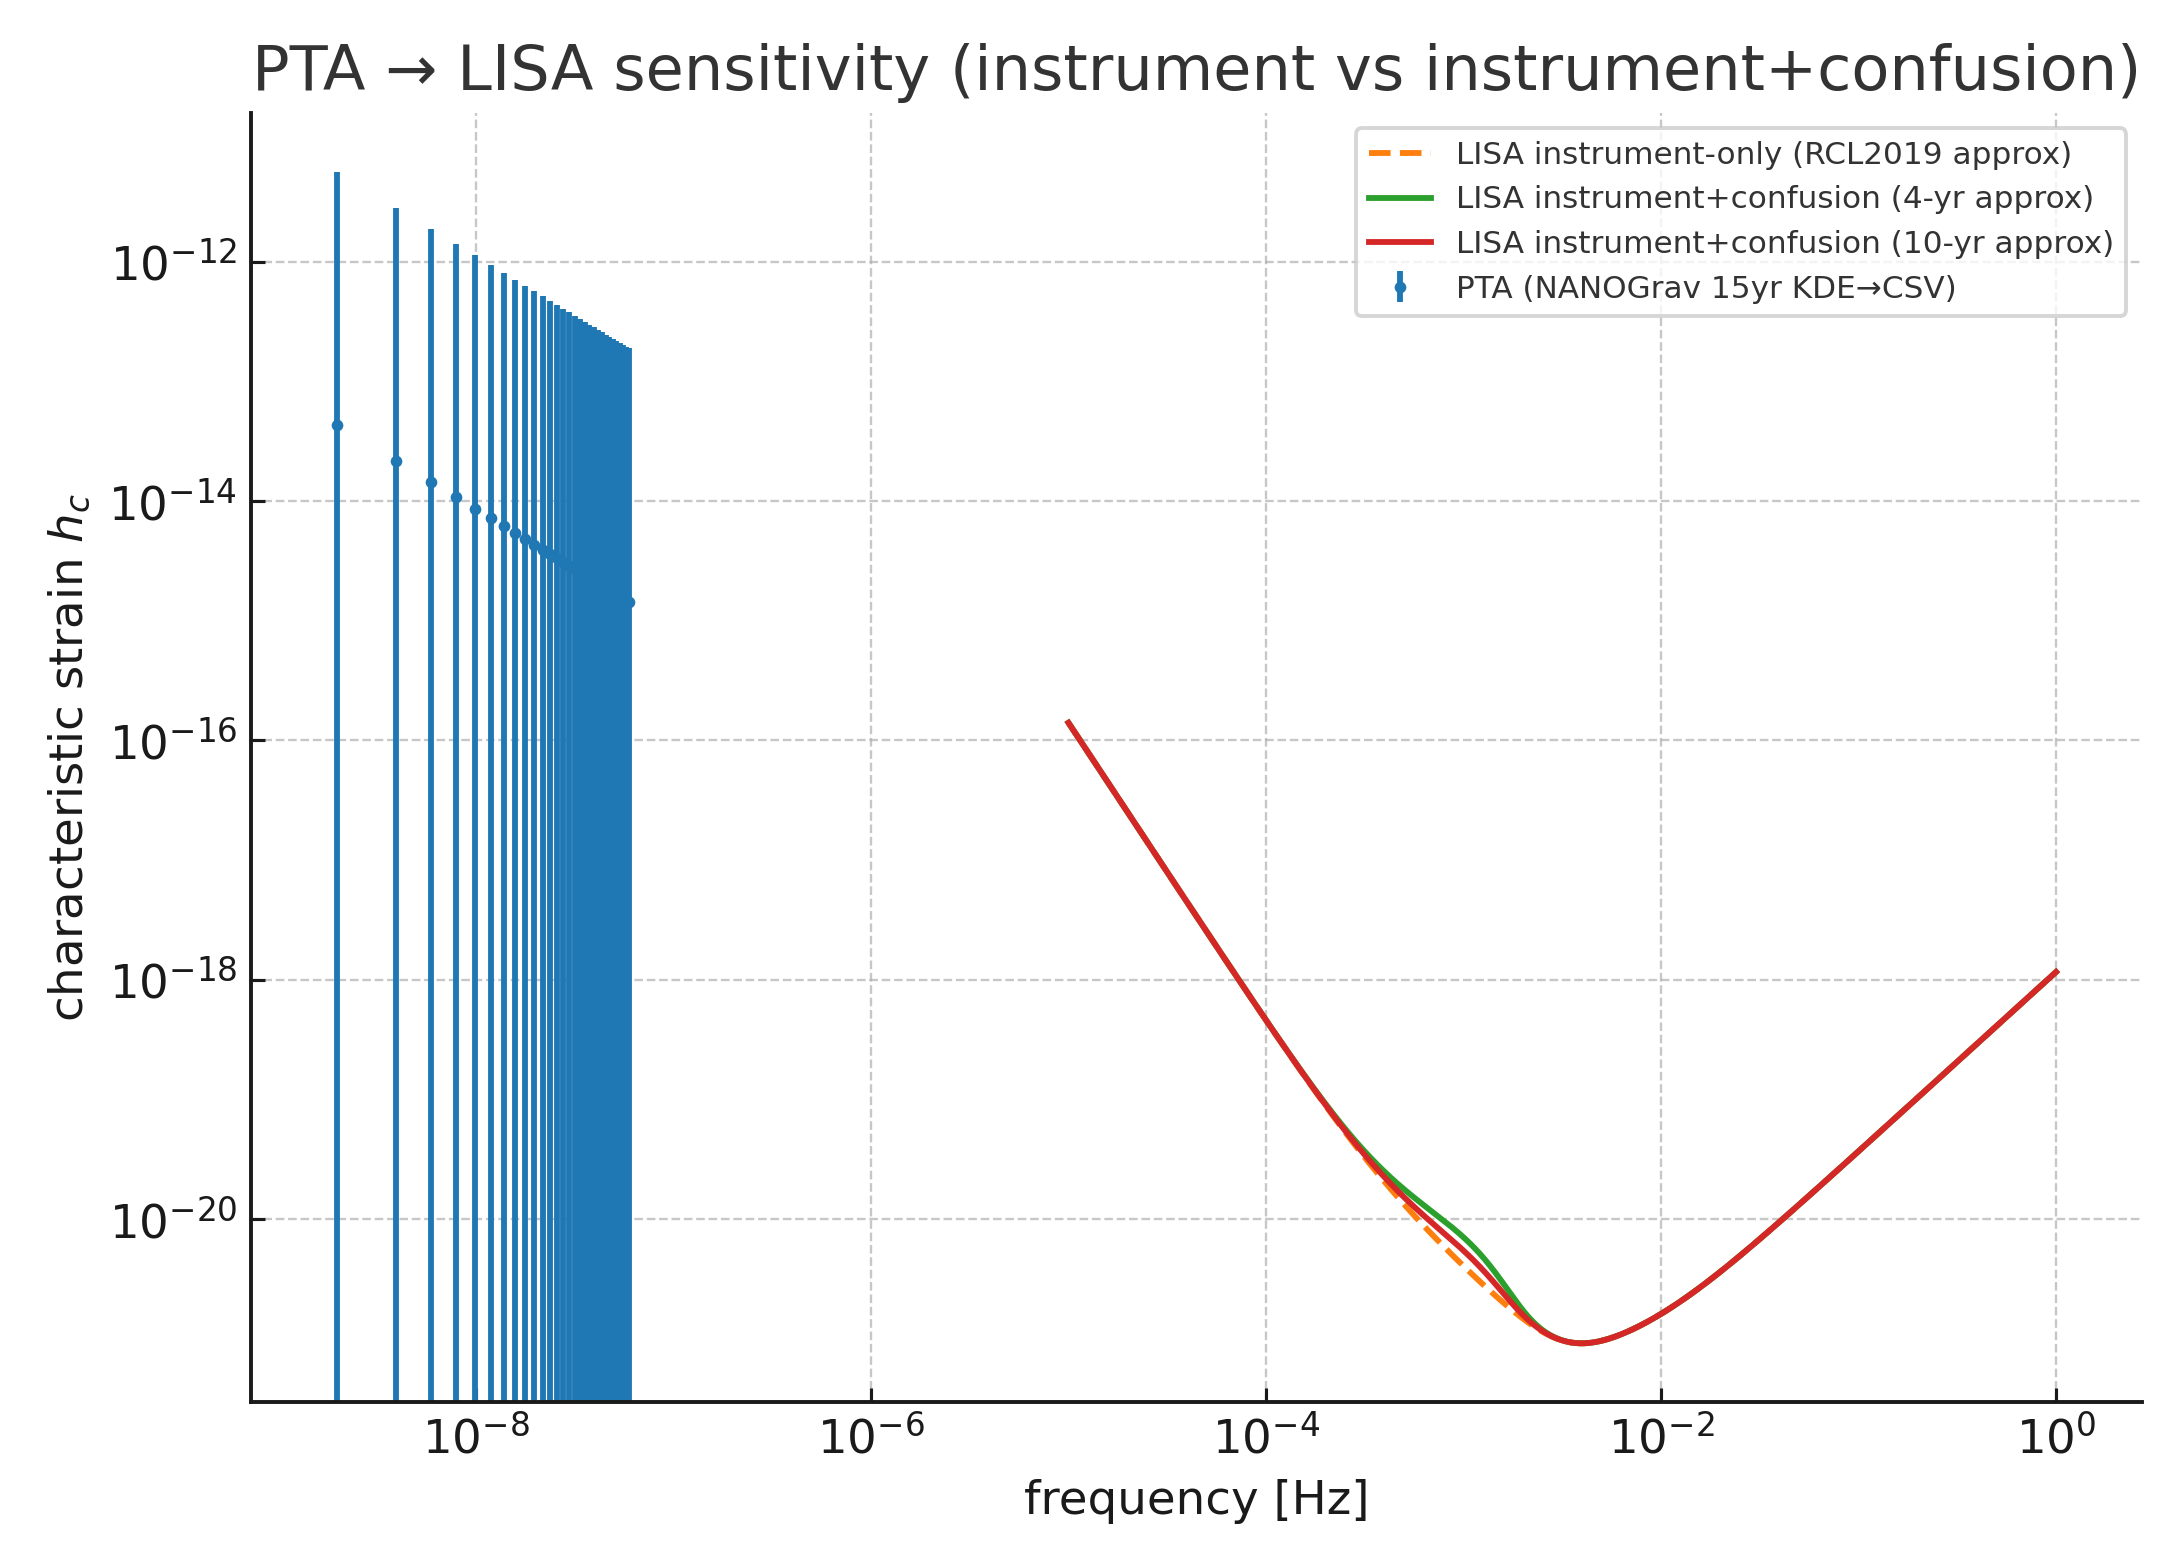
\includegraphics[width=0.46\textwidth]{figures/PTA_LISA_overlay_instrument_vs_confusion_20250812_235811.png}
  \caption{PTA$\to$LISA instrument-only vs instrument+confusion (4y/10y).}
\end{figure}

\bibliographystyle{apsrev4-2}
\bibliography{refs}
\end{document}
